%A good requirement is:
%*Correct
%*Unambiguous (all statements have exactly one interpretation)
%*Complete (where TBDs are absolutely necessary, document why the information is unknown, who is responsible for resolution, and the deadline)
%*Consistent
%*Ranked for importance and/or stability
%*Verifiable (avoid soft descriptions like “works well”, “is #user frndly”; use concrete terms and specify measurable #quantities)
%*Modifiable (evolve the Requirements Specification only via a #formal change process, preserving a complete audit trail of #changes)
%*Does not specify any particular design
%*Traceable (cross-reference with source documents and spawned documents).




\chapter{Requirement specification}
This chapter describes both functional aswell as general system requirements.
\section{General description}

\subsection{General System}
\begin{figure}[H]
	\centering
	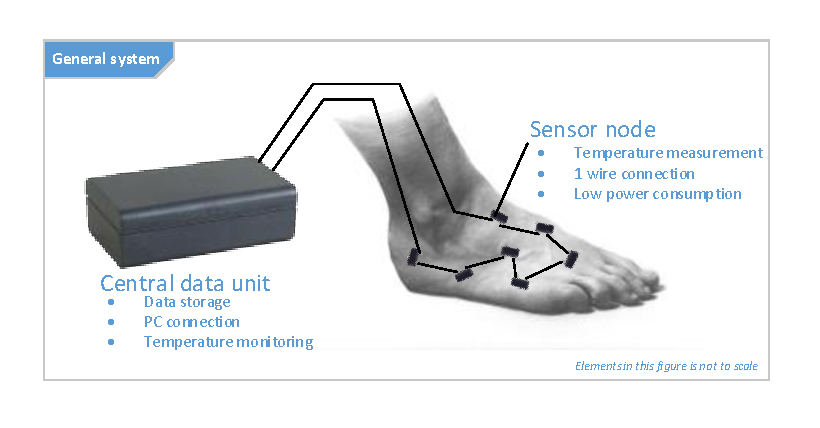
\includegraphics[width=1\textwidth]{billeder/GeneralSystem}
	\caption{General System}
\end{figure}

\subsection{General system description}
The system will be mounted on and around the foot of a person who is likely to develop Charcot foot. The system will capture data from temperature sensors which can be used to determine whether there is a danger of overloading the foot and/or joint.

\subsubsection{Central data unit description}
The Central data unit communicates with the sensor nodes to collect data from each node. This data is stored on the CDU's memory with a time stamp and sensor node identifier.\\
The CDU can transfer the data to a computer. This communication can be wired or wireless but this may be implemented solely as a feature for this project and not the final product.

\subsubsection{Sensor node description}
The sensor node is in general a generic sensor which contains two functionalities. It contains the custom power line communication protocol and it can measure data. This measurement can be temperature, accelerometer value etc. The nodes gets both power and communication via. the one wire and it is then daisy chained to the next sensor and so forth until the wire ends in the CDU again. This helps minimize wires in the insole/sock and simplifies the system. 

\subsection{Constraints}
\textit{Currently none.}
\subsection{Dependencies}
\textit{Currently none.}

%\subsection{Prototype af UI eller GUI}

%\subsection{Beskrivelse af UI eller GUI}

%\section{General system functionality}
%The systems function that does not include user input will be explained here in a non technical way and then later on be described technically in the architecture and design documents.\\
%This section serves to describe the system functionality
%\textbf{CDU}\\
%The CDU is the central part of this system. It handles the communication protocol as well as the data transmitted. The data is saved in internal memory. When the system starts the CDU initiates by contacting every address in a defined range on the communication line. As sensors respond with their type, their type and address are saved in memory. When the whole range has been contacted the system starts normal operation mode. In normal mode the system contacts every system at least one time every minute. The data is saved in the CDUs memory. \\
%\textbf{Sensor}\\
%The sensor nodes have an address and a type. The type is either an activity sensor or a temperature sensor. The addresses are hard-coded into the sensor. The sensors have data ready when the CDU asks for data. The sensors are powered from the communication line.\\
%\textbf{Communication and protocol}\\
%The protocol consist of a wire connected to all the sensors in a daisy chain. The CDU controls the line and maintains the connection. The CDU initiates communication and retrieves data from the line.\\

\section{Functional requirements}
Below is listed all functional requirements to the system.\\

\subsection{Use Case diagram}
Below is shown the use case diagram.\\

\begin{figure}[H]
\centering
\includegraphics*[width=.7\textwidth]{billeder/UseCase_vector}
\label{usecase_fig}
\caption{Use case diagram}
\end{figure}

\subsection{Actors of the system}

\subsubsection{Primary actors}

\begin{table}[H]
	\centering
	\begin{tabular}{|l|p{7cm}|}
	\hline
	Actor name & Patient \\ \hline
	Type & Primary \\ \hline
	Description &  The patient set the system to run and initiates data extraction from the CDU.\\ \hline
	\end{tabular}
\end{table}

\subsubsection{Secondary actors}

\begin{table}[H]
	\centering
	\begin{tabular}{|l|p{7cm}|}
	\hline
	Actor name & Computer \\ \hline
	Type & Secondary \\ \hline
	Description & The computer can extract data from the Central data unit. It is not intended as a control unit but mostly just for demonstration and debug purposes. \\ \hline
	\end{tabular}
\end{table}

\subsection{Use Cases}

\subsubsection{Set system to normal operation}

\begin{table}[H]
	\centering
	\begin{tabular}{|l|p{10cm}|}
	\hline
	Goal 							& To set the system to normal operation. \\ \hline
	Initialisation 					& The Patient initiates the use case. \\ \hline
	\multirow{1}{*}{Actors} 		& Patient \\ 
 \hline
	Reference 						& none \\ \hline
	\# of concurrent events 		& 1 \\ \hline
	Prerequisite  					& The patient connect the sensors to the port on the CDU. \\ \hline
	Post condition 					& The system is set to normal operation. \\ \hline
	\multirow{2}{*}{Main Scenario} 	& 1. The patient clicks the  "ON"-button. \\
	& 2. The system indicates successful start up.\\ \hline
	\multirow{2}{*}{Exceptions} & 2a. The system does not indicate sucessful start up. \\
	& - The patient contacts technical support. \\ \hline
	\end{tabular}
\end{table}

\subsubsection{Extract data from CDU}
\begin{table}[H]
	\centering
	\begin{tabular}{|l|p{10cm}|}
	\hline
	Goal 							& Extract the data from CDU.\\ \hline
	Initialisation 					& The patient connects the CDU to a computer. \\ \hline
	\multirow{2}{*}{Actors} 		& Patient \\ 
									& Computer \\\hline
	Reference 						& None \\ \hline
	\# of concurrent events 		& 1 \\ \hline
	Prerequisite  					& None \\ \hline
	Post condition 					& The data has been transferred to a computer. \\ \hline
	\multirow{4}{*}{Main Scenario} 	& 1. The patient disconnects the CDU from the sensors and connects it to the computer. \\
									& 2. The patient opens the program to transfer data.\\
									& 3. The patient sets up the program and sends the transfer command.\\ 
									& 4. The CDU responds with the data. \\ \hline
	\multirow{4}{*}{Exceptions} & 4a. The CDU does not respond. \\ 
								& - The CDU and computer are not connected correctly.\\											& 4b. The CDU responds "There is no data". \\
								& - There is not data on the CDU to respond with.\\\hline
	\end{tabular}
\end{table}


%\section{Non functional requirements}
%Below is listed all non-functional requirements. \\

\subsection{General requirements}
\begin{table}[H]
\begin{tabular}{p{10cm} p{2cm}}
$\bullet$ The system should be simple and as comfortable as possible for the patient. & \\
$\bullet$ The system should be small enough to have on a belt or similar and in a sock or insole. &\\
\end{tabular}
\end{table}


\subsection{Sensor requirements}

\subsubsection{Functionality Requirements}
\begin{table}[H]
\begin{tabular}{p{8cm} p{5cm}}
$\bullet$ Temperature accuracy: & <$0.5^o$C\\
$\bullet$ Measurement rate: & min. once per CDU cycle\\
\end{tabular}
\end{table}

\subsubsection{Hardware Requirements}
%Krav til hardware (if any)\\
\begin{table}[H]
\begin{tabular}{p{8cm} p{2cm}}
$\bullet$ Power consumption: & <0.05W\\


\end{tabular}
\end{table}


\subsubsection{Software Requirements}
%Krav til software (if any)\\
\begin{table}[H]
\begin{tabular}{p{8cm} p{2cm}}
$\bullet$ & None\\


\end{tabular}
\end{table}


\subsubsection{External interfaces}
\begin{table}[H]
\begin{tabular}{p{8cm} p{2cm}}
$\bullet$ Custom power line communicatin bus: & Yes\\
$\bullet$ Wires in: & 1\\
$\bullet$ Wires out: & 1\\
\end{tabular}
\end{table}

\subsection{Central data unit requirements}

\subsubsection{Functionality Requirements}
\begin{table}[H]
\begin{tabular}{p{8cm} p{2cm}}
$\bullet$ Cycle\footnotemark: & 1 min\\
\end{tabular}
\end{table}
\footnotetext{In a cycle the CDU will collect data once from all sensors}
\subsubsection{Hardware Requirements}
%Krav til hardware (if any)\\
\begin{table}[H]
\begin{tabular}{p{8cm} p{5cm}}
$\bullet$ Power consumption: & <0.5W \footnotemark \\
$\bullet$ Memory: & 24 hours of data collection ($\sim$152kB) 256kB suggested.\\
$\bullet$ Real time clock: & Yes\\
\end{tabular}
\end{table}
\footnotetext{Sensor supply excluded}


\subsubsection{Software Requirements}
%Krav til software (if any)\\
\begin{table}[H]
\begin{tabular}{p{8cm} p{5cm}}
$\bullet$ Save entries must contain: &Sensor identifier. \\
~ 									&Temperature. \\
~									&Timestamp. \\
~									&Type. \\
~									&Erros. \\
\textit{The order doesn't need to follow the above order.}

\end{tabular}
\end{table}


\subsubsection{External interfaces}
\begin{table}[H]
\begin{tabular}{p{8cm} p{2cm}}
$\bullet$ Custom power line communication bus: & Yes\\
$\bullet$ CDU to computer interface: & Yes\\
\end{tabular}
\end{table}

\subsection{Project requirements}

\subsubsection{Documentation}
\begin{itemize}
\item English
\item SysML
\end{itemize}

\subsubsection{Technologies and tools}
\begin{itemize}
\item Matlab
\item Maple/Mathcad
\item Microsoft Visio 2010/2013
\item TortoiseSVN
\item TeXmaker
\item Modelsim
\item Quartus 12.1
\item MPLAB X
\end{itemize}

\subsubsection{Misc}
\begin{itemize}
\item Documentation and final assignment is written in LaTeX.
\end{itemize}

